%
% File naaclhlt2016.tex
%

\documentclass[11pt,letterpaper]{article}
\usepackage{naaclhlt2016}
\usepackage{times}
\usepackage{latexsym}
\usepackage{graphicx}
\usepackage{subfigure} 
\usepackage{balance}
\usepackage{hyperref}
\usepackage{natbib}
\usepackage{arydshln}

\newcommand{\squishlist}{
   \begin{list}{$\bullet$}
    { \setlength{\itemsep}{-1pt}      \setlength{\parsep}{3pt}
      \setlength{\topsep}{1pt}       \setlength{\partopsep}{0pt}
      \setlength{\leftmargin}{1.5em} \setlength{\labelwidth}{1em}
      \setlength{\labelsep}{0.5em} } }
\newcommand{\squishend}{
    \end{list}  }
    
%\naaclfinalcopy % Uncomment this line for the final submission
\def\naaclpaperid{***} %  Enter the naacl Paper ID here
 
\newcommand\BibTeX{B{\sc ib}\TeX}

\title{Machine Teaching for Information Extraction}

\author{Author 1\\
	    XYZ Company\\
	    111 Anywhere Street\\
	    Mytown, NY 10000, USA\\
	    {\tt author1@xyz.org}
	  \And
	Author 2\\
  	ABC University\\
  	900 Main Street\\
  	Ourcity, PQ, Canada A1A 1T2\\
  {\tt author2@abc.ca}}

\date{}

\begin{document}

\maketitle

\begin{abstract}
 Traditional machine learning has focused on algorithms, and typically require long and complex iterations (often with an ML expert in the loop) to develop a final model. In contrast, Machine Teaching focuses on the user, and how to most effectively leverage him/her for a given learning task. Prior work suggests that a user is most effective when model updates are rapid, focused, and incremental, and that paying attention to this can dwarf minor algorithmic improvements in the learning algorithms themselves.
 
With this in mind, we have developed IKE (Interactive Knowledge Extraction), an extraction tool that performs fast, interactive bootstrapping to develop high-quality extraction patterns for targeted relations. It allows quick exploration of the pattern space, and automatically suggests possible new patterns to explore based on relation mentions collected so far. 

Our evaluation suggests that relation tables can be populated substantially faster than manual pattern authoring method while retaining accuracy, and that the machine-learning-based relation suggester significantly improves the performance of the tool. We are using IKE to develop a Knowledge Base (KB) of semantic knowledge to help answer 4th Grade Science questions in Project Aristo.
\end{abstract}

%-------------------------------------------------------

\begin{figure*}[th]
\begin{center}
   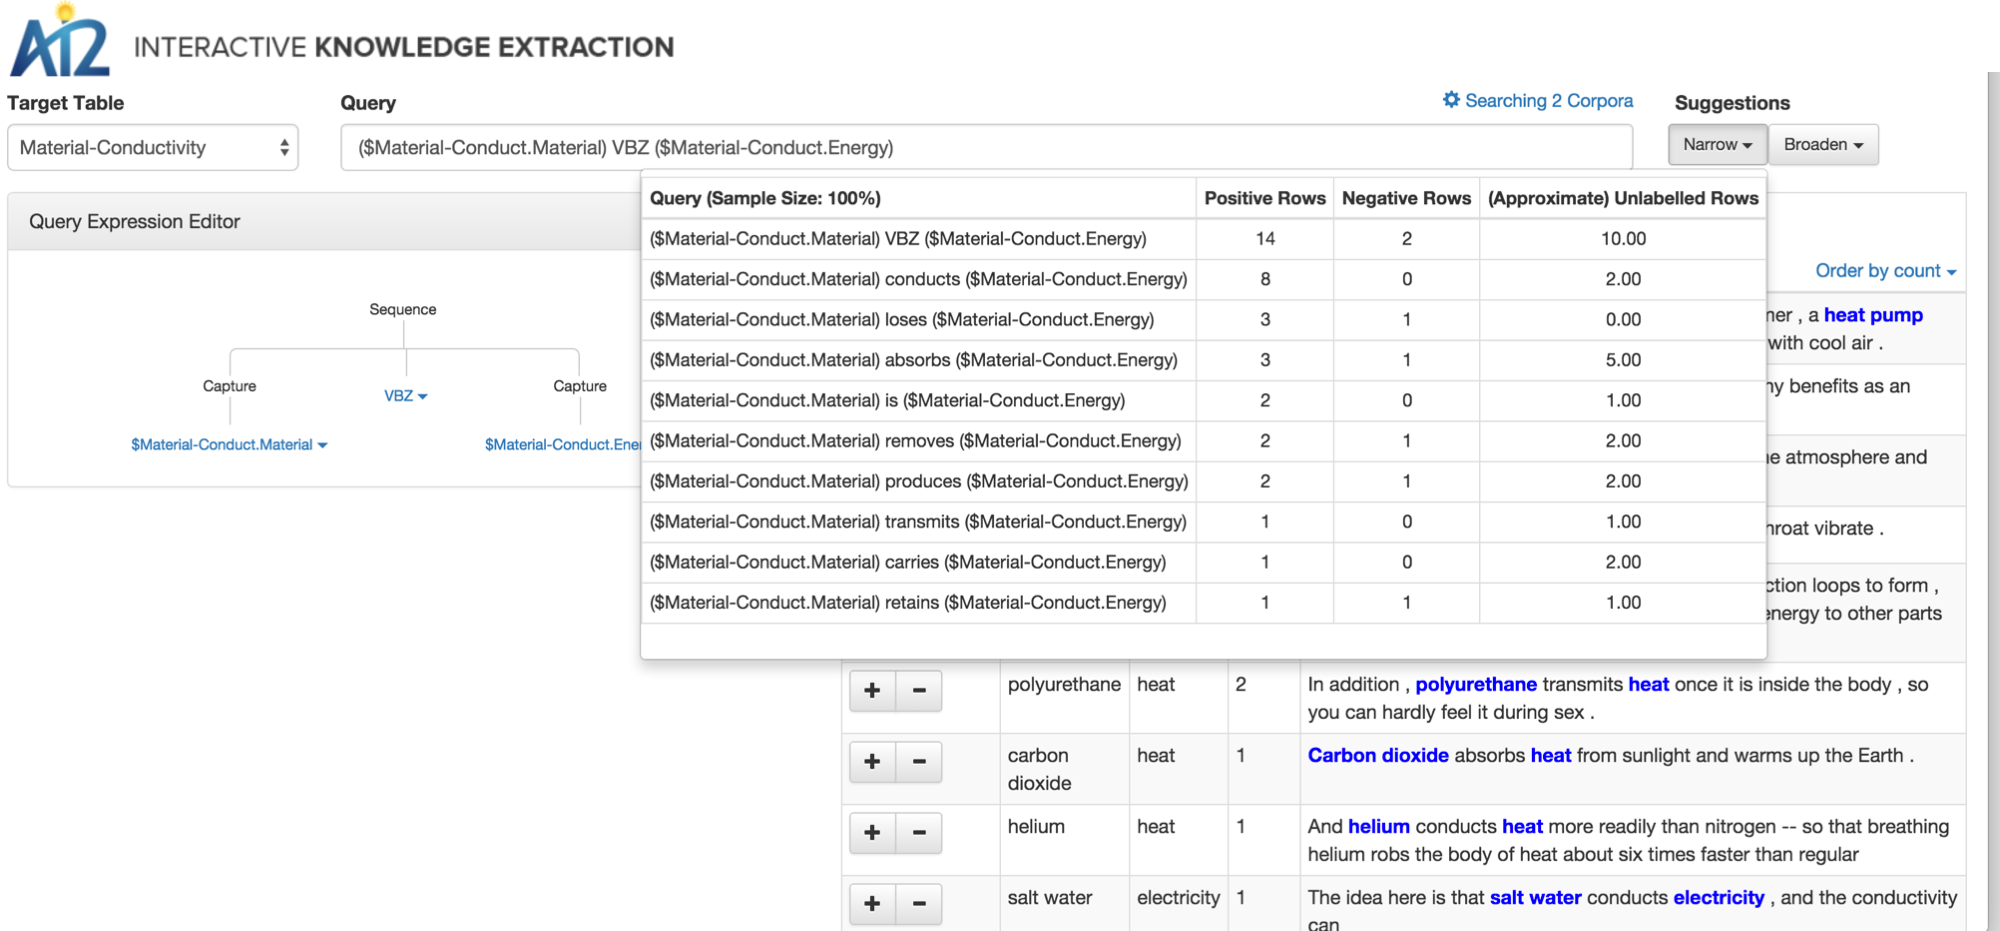
\includegraphics[scale =.5] {./figures/IKE_query_suggestions_narrow_2.pdf}
\caption{Example of IKE query suggestions}
\label{fig:IKE-query-suggest}
\end{center}
\end{figure*}

\section{Introduction}
Any system that wants to work with structured knowledge needs an efficient and reliable way acquire it; extraction from text is an obvious approach. In project Aristo, we are building a computer system that can answer elementary grade science exam questions.    Many of these questions require inference with some form of structured knowledge. 
 
Automatic open information extraction algorithms (e.g., \cite{Angeli2015LeveragingLS}) are efficient, however they produce noisy results (e.g., best F1 score of 28.3 for the KBP slot filling task as reported in  \cite{Angeli2015LeveragingLS}). Weakly supervised automatic bootstrapping methods \cite{Carlson:wsdm2010,Gupta2014ImprovedPL} are very precise in the initial bootstrapping iterations, but  digress in the later iterations, a problem generally referred to as semantic drift. These approaches are limited to binary relation extraction.
 
There have been recent attempts at more interactive methods, which can be seen as ``Machine Teaching'' \cite{Amershi2014PowerTT,Amershi2015ModelTrackerRP} approaches to KB construction. The premise here is that a focus on the user can dwarf minor algorithmic improvements in the ML algorithms themselves.
Soderland et al.~\cite{Soderland2013OpenIE} showed that users can be surprisingly effective at authoring and refining extraction rules for a slot filling task. Hoffmann et al.~\cite{Hoffmann2015ExtremeEO} build on this work to create an interactive extraction tool, InstaRead, allowing user-in-the-loop bootstrapping.
These earlier proposed techniques are restricted to binary relations, user is expected to author dependency parse based patterns, and relation arguments are often named entities of type person, location, organization etc.

In this paper, we take the machine teaching approach further and present IKE, a new tool for interactive knowledge extraction. Our approach is novel in the sense it allows us to extract n-ary relations between any phrases, and it is targeted towards a domain expert in the topic of relations to be built, and not a linguistic expert. E.g., a user who has elementary grade science knowledge should be able to build a KB for Aristo. 

IKE takes care of all the linguistic processing including POS tagging, chunking, indexing and computing co-occurrence statistics of patterns from a large dataset. It supports fast, interactive bootstrapping and includes several novel features including a simple but rich pattern language, use of embedding-based similarity measures for extraction, support for N-ary relations, support for user-defined data types, and an easy-to-use interface. 

IKE is interpretable at each step.
The pattern queries discovered by the system are transparent to the user in terms of why the system thinks these patterns are useful. Please refer to Figure \ref{fig:IKE-query-suggest} for a sample screenshot of IKE query suggest. 
 For each suggested query, it provides number of positive, negative and unlabeled instances each query would retrieve. User can accept, refine or reject these suggestions, to continue iterative relation learning. 
  Similarly, for each relation instance extraction it shows the evidence from the corpus in terms of sentences which contributed to this extraction. 
If the user chooses to use the system suggested queries without any intervention, he/she can still annotate candidate relation instances proposed in each iteration which are used to come up with better patterns in the next iteration. 

  
Rest of the paper is organized as follows: In Section \ref{sect:IKE-description} we describe the workflow of creating a knowledge table using the proposed IKE techniques. 
Preliminary experimental results are presented in Section \ref{sect:expt-eval} followed by conclusions in Section \ref{sect:conclusions}.

%-------------------------------------------------------
\begin{figure*}[bth]
\begin{center}
   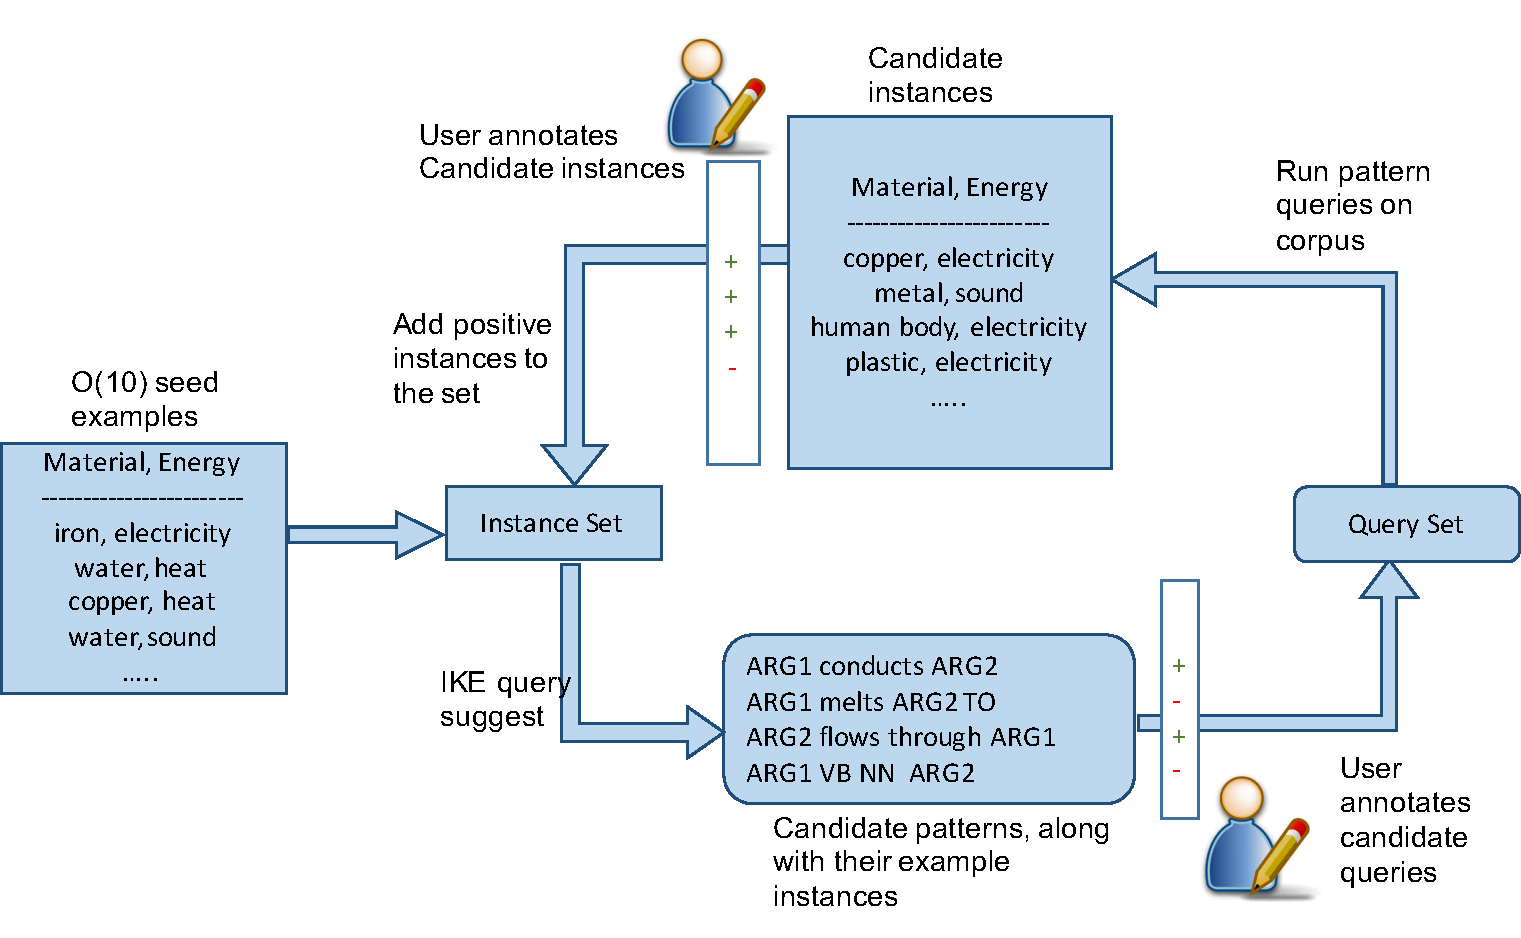
\includegraphics[scale =.5] {./figures/IKE_bootstrapping_ME_1.pdf}
\caption{IKE interactive bootstrapping work-flow to create Material-Conductivity table}
\label{fig:IKE-Bootstrapping}
\end{center}
\end{figure*}

\section{Interactive Knowledge Extraction (IKE)} \label{sect:IKE-description}

\subsection{Overview}
IKE is an interactive tool with the following important features:
\squishlist
 \item pattern-based search over a corpus
 \item rich query language
 \item embedding-based list expansion
 \item easy annotation of results
 \item automatic query suggestion
 \item support for entity types
\squishend
Next we describe a typical workflow with IKE, and how these features are used. 
    
\subsection{Target Relation Extraction Workflow} \label{sect:IKE-workflow}
IKE provides a search interface over the corpus. User can issue a regular expression query over the indexed corpus, and get back results grouped by captcha groups within the  query. E.g., a query ``(NP) can conduct (NP)'' will return a set of noun phrase pairs separated by context ``can conduct''. 
IKE uses BlackLab \cite{blacklab-tool} for indexing the corpus. This results in a rich query language supporting wildcards, window sizes, POS tags, chunk tags, as well as any existing IKE built knowledge tables. Next, we explain the IKE features in the context of building an example target relation ``MATERIAL conducts ENERGY''.

%Describe the method to create type tables
\subsubsection{Creating the Material Energy types}
IKE lets a user build single column tables or dictionaries that can act as types. E.g., while building ``Conducts'' table, user can first build a list of ``Materials'' and ``Energies'' separately, by starting with few seed examples and then using word2vec based expansion to expand the list. 
E.g., query ``(\$MaterialList $\sim$ 100)'' would retrieve 100 phrases that are similar to materials already present in the list.

\subsubsection{Creating the initial conducts table}
Once these 2 dictionaries are built (e.g. ``MaterialList'' ``EnergyList''), then while creating the binary relation Conducts we can use queries like these ``(\$MaterialList) conducts (\$EnergyList)'', or `` (\$EnergyList) flows through (\$MaterialList)'' to extract pairs of materials and energies they conduct. This would let us create a high precision seed table.

\subsubsection{Bootstrapping to retrieve more instances of Conducts relation}
IKE lets a user build a knowledge relation using an interactive bootstrapping approach. An example work-flow to build ``MaterialConductivity'' relation is illustrated in Figure \ref{fig:IKE-Bootstrapping}. The high precision seed table is used as input to find additional patterns (queries) to extract the target relation. These patterns are then used to find  more instances of the relation. User can interact with the system to increase the precision of query and instance sets.

Note that in this process, IKE churns all occurrences of labeled instances and comes up with context patterns useful to extract the target relation. Though the queries can look complicated with POS and chunk tags within them, user need not author them by hand. Hence the required skill set and data analysis workload on user is significantly reduced.
The system still gives the control in user's hand by letting him/her filter/edit the queries, and annotate the extractions in each iteration. This method is referred to as ``\emph{IKE}'' in  Section \ref{sect:expt-eval}. 

IKE's query suggestions feature makes use of  the human annotations for a relation, to refine (either narrow or broaden) user's queries. The narrow feature would restrict the user query e.g. replacing a POS tag with a specific word, whereas the broaden feature generalizes the given user query e.g. replacing a word by its POS tag. In both cases the candidate queries are ranked based on the number of positive, negative, and unlabeled instances it produces.
Figure \ref{fig:IKE-query-suggest} shows an example of narrowing a query for Conducts table, IKE suggests most common verbs found in the corpus, ranked by their co-occurrence with as many positive and as fewer negative examples as possible. 

%\subsection{IKE System Details}
%a brief paragraph on implementation, e.g., we use Blacklabs, we prefilter the corpus, ...? 

%-------------------------------------------------------

\section{Experimental Evaluation} \label{sect:expt-eval}
Our goal is to evaluate the degree to which IKE helps to acquire relations in terms of precision, yield, and time. To do this, we compare our interactive IKE extraction approach (described in Section \ref{sect:IKE-description}) with two alternative methods: manual and fully automatic (AKBC). These approaches can also be run in IKE by disabling certain features and using a different workflow:

\squishlist
\item \emph{Manual}: In this method user makes use of IKE just to run the pattern based search over corpus. Patterns are manually authored. Patterns can be refined looking at the search results. Set expansion, and query suggestion features are not used. 
\item \emph{Automatic}: This method takes as input a seed relation table with few entries, and lets the system bootstrap on its own, without any further interaction. Both user annotation steps in the Figure \ref{sect:IKE-workflow} are replaced by adding all patterns and instances that occur at least $k$ times in the corpus. We used $k$ = 2 for the experiments in this section.
\squishend

We compare IKE with these alternative method for building following target relations: (Animal, BodyPart),  (Material, Conducts), and (Pollutant, Type of Pollution). All methods make use of following four science text corpora (\#sentences in the parenthesis): Barron's study-guide for 4th grade science (1.2K), CK-12 corpora (17K), Simple Wikipedia ($\sim$1M), and Science subset of Waterloo corpus ($\sim$1.5M) \cite{waterloo-corpus}.

\begin{table}[tbh]
\centering
\boldmath
\scalebox{0.75}{%
 \begin{tabular}{l|cc|c|cc} %\hline
Method & \multicolumn{2}{c|}{\#Instances  (yield) } & Precision & \multicolumn{2}{c}{Time } \\
\cline{2-3} \cline{5-6}
 & Total & Positive & in \% & \#queries & in min.\\ \hline
\emph{Manual}     &24  & 16  & 66.7 & 5   & 30 \\
\emph{Automatic}  &183 & 63  & 34.4 & 108 & -\\ \hdashline
\emph{IKE}        &142 & 84  & 59.2 & 41  & 20\\ %\hline
%(Manual + word2vec)   &34  & 24 & 10  & 70.6 & 7 \\
\end{tabular}
}
\caption{Relation (``MATERIAL'' conducts ``ENERGY''): Comparison of three types of extraction methods.} \label{table:conducts}
\end{table}

\begin{table}[tbh]
\centering
\boldmath
\scalebox{0.75}{%
 \begin{tabular}{l|cc|c|cc} %\hline
Method & \multicolumn{2}{c|}{\#Instances  (yield)} & Precision &   \multicolumn{2}{c}{Time } \\
\cline{2-3} \cline{5-6}
   & Total & Positive  & in \% & \#queries & in min.\\  \hline
\emph{Manual}           & 291  & 61 & 21.0 & 11 & 40\\
\emph{Automatic}        & 1386 & 48 & 3.4 & 228& - \\ \hdashline
\emph{IKE}              & 249  & 143& 57.4& 21 & 30 \\ %\hline
\end{tabular}
}
\caption{Relation (``ORGANISM'' has ``BODYPART''): Comparison of three types of extraction methods.} \label{table:body-parts}
\end{table}

Table \ref{table:conducts} shows the comparison for "MATERIAL conducts ENERGY" relation.
We can see that manual method yielded 16 positive instances of this relation with 66.7\% precision using 5 manually authored queries and took 20 minutes. Fully automated method produced many more instances (184) but with poor precision (33\%) resulting in 63 positive relation instances. This method is fastest among all. IKE method makes use of both interactive and machine learning features to produce 142 instances (84 positive) with reasonable precision (60\%) and takes less time than manual method. 

Table \ref{table:body-parts} shows similar comparison for Organism-BodyParts relation. These preliminary results indicate that \emph{Manual} method is high precision, low recall whereas \emph{Automatic} method is low precision high recall. \emph{IKE} gives best of both worlds to increase the yield of manual method
in similar amount of time and maintaining reasonable precision.

**** \textbf{an example of n-ary relation with general phrases (Animal, Adaptation, Challenge), where adaptation is ``ADJ BODYPART''}

%-------------------------------------------------------

\subsection*{Future research directions}
Currently IKE is trying to learn best extraction patterns for a target relation using manual annotations of instances and patterns. There is a possibility of improvement in the sense that the query suggestions for a relation can be based on a model for both arguments along with context between and around them. 
%-------------------------------------------------------
%\newpage
%\clearpage

\section{Conclusions}  \label{sect:conclusions}
In this paper we presented IKE (Interactive Knowledge Extraction) technique that performs fast, interactive bootstrapping to develop high quality extraction patterns for targeted relations. We compared IKE to manual pattern authoring and completely automatic extraction variants. Preliminary experiments are encouraging and show that IKE makes the best of both worlds by improving recall of manual extraction process while retaining precision within acceptable bounds.

IKE tool is an example of a machine teaching system where system can do quick exploration of the pattern space to automatically suggest possible new patterns, and user can annotate/edit/add patterns as well as annotate proposed relation instances. In the next iteration, the ML system makes use of user annotations to generate better patterns. Thus, IKE enables interpretable knowledge extraction from large corpora under user's guidance.



%-----------------------------

\subsubsection*{Acknowledgments:} 

%\clearpage
%\newpage
\bibliography{references}
\bibliographystyle{abbrv}

\end{document}